\documentclass[finals,table,dvipsnames,11pt]{beamer}
\usefonttheme{professionalfonts}

\usepackage[english]{babel}
\usepackage[utf8]{inputenc}
\usepackage[T1]{fontenc}
\usepackage{amsmath}
\usepackage{multicol}
\usepackage{graphicx}
\usepackage{hyperref}
\usepackage{float}
\usepackage{url}
\usepackage{wasysym}
\usepackage{xspace}
\usepackage{times}
\usepackage{booktabs}
\usepackage{xcolor}
\usepackage{marvosym}
\usepackage{tikz}
\usepackage{listings}
\usepackage{fancybox}
\usepackage{shadow}


\usetikzlibrary{arrows,shapes,backgrounds}
\tikzstyle{every picture}+=[remember picture]
\tikzstyle{na} = [baseline=-.5ex]

\DeclareGraphicsExtensions{.eps,.pdf,.JPG,.jpg,.jpeg,.png,.PNG}
\graphicspath{
{./figures/}
}
\definecolor{sdnblue}{HTML}{005baa}
\definecolor{sdngrey}{HTML}{646464}

\setbeamertemplate{navigation symbols}{}
\setbeamercolor{title}{fg=sdnblue}
\setbeamertemplate{footline}[frame number]
%\setbeamercolor{background canvas}{bg=black!95}
%\setbeamercolor{normal text}{bg=black,fg=white}
\setbeamercolor{frametitle}{fg=sdnblue}
%\setbeamercolor{section in sidebar}{fg=blue!70}
%\setbeamercolor{sidebar}{fg=black}
%\setbeamercolor{structure}{bg=black,fg=black!5}
%\setbeamercolor{item projected}{fg=black,bg=white}


\setbeamertemplate{items}[square] 
\setbeamertemplate{caption}[numbered]
\setbeamerfont{caption}{size=\scriptsize,family=\it}
\usefonttheme{professionalfonts} % using non standard fonts for beamer
\usefonttheme{serif} % default family is serif

%--------------------------------
\hypersetup{bookmarksopen=true,
bookmarksnumbered=true,  
pdffitwindow=true, 
pdfstartview=Fit,
%pdfpagemode=FullScreen,
pdffitwindow=true,
pdftoolbar=true,
pdfmenubar=true,
pdfwindowui=true,
pdfauthor={Alexander Barth{,} Aida Alvera-Azc\'{a}rate{,} Mohamed~Ouberdous{,} Charles~Troupin{,} Sylvain~Watelet \& Jean-Marie~Beckers},
pdfsubject={DIVA Lecce 2016},
pdftitle={DIVA Lecce 2016},
bookmarksopenlevel=0,
colorlinks=true,
linkcolor=blue,anchorcolor=black,%
citecolor=blue,filecolor=black,%
menucolor=black,urlcolor=blue,%
pdfpageduration=1,%
pdffitwindow=true
}

\logo{\vspace{-5mm}
\includegraphics[height=0.5cm]{gherlogo_transparent}~
\includegraphics[height=0.5cm]{Logo_SeaDataNet_fond_transparent}\hspace{7mm}}

\author[Alexander Barth, Aida Alvera-Azc\'{a}rate, Mohamed~Ouberdous, Charles~Troupin, Sylvain~Watelet \& Jean-Marie~Beckers]{Alexander Barth, Aida Alvera-Azc\'{a}rate, Mohamed~Ouberdous,\\
 Charles~Troupin, Sylvain~Watelet \& Jean-Marie~Beckers}
  
\title[]{\diva Lecce 2016}
\date{Lecce (Italy), 11--14 April 2016}


%--------------------------------

\definecolor{colorcite}{rgb}{0,.46,.46}
\newcommand{\diva}{\textsf{Diva}\xspace}
\newcommand{\mat}{\mathbf}
\newcommand{\important}[1]{\textcolor{sdnblue}{#1}}
\newcommand{\method}[1]{\textcolor{gray}{#1}}
\newcommand{\tool}[1]{\textcolor{sdngrey}{\texttt{#1}}}
\newcommand{\nablab}{\boldsymbol{\nabla}}
\newcommand{\ddiff}{\mbox{d}}
\newcommand{\cita}[1]{\textcolor{colorcite}{#1}}
\newcommand{\fleche}{$\rightarrow$\,}
\newcommand{\snr}{\lambda}
\newcommand{\noise}{\epsilon}

\newcommand{\directory}[1]{\texttt{\color{ForestGreen}{#1}}}
\newcommand{\file}[1]{\texttt{\color{MidnightBlue}{#1}}}
\newcommand{\command}[1]{\texttt{\color{RedOrange}{#1}}}
\newcommand{\resfile}[1]{\texttt{\color{MidnightBlue}{#1}}}

\newcommand{\statmean}[1]{\left\langle #1 \right\rangle}
\newcommand{\true}[1]{{#1}^t}
\newcommand{\analyzed}[1]{{#1}^a}
\newcommand{\observation}{ \mbox{\boldmath   $ \protect\mathrm{y} $} }
\newcommand{\forecasted}[1]{{#1}^f}
\newcommand{\kalmangain}{\matr{K}}
\newcommand{\Hobs}{\matr{H}}
\newcommand{\errorv}{\vect{\epsilon}}
\newcommand{\errorobs}{\vect{\epsilon}^o}
\newcommand{\Perr}{\matr{P}}
\newcommand{\Rerr}{\matr{R}}

\newcommand{\matr}[1] { \mbox{\boldmath   $ \protect\mathsf{#1} $} }
\newcommand{\trcon}[1]{{#1}^\star}
\newcommand{\adj}[1]{\trcon{#1}}
\newcommand{\elem}[2]{\left( #1 \right)_{#2}}
\newcommand{\trace}{\operatorname{trace}}
\newcommand{\sing}{\rho}

\newcommand{\myshadowbox}[1]{\shabox{\parbox{10cm}{#1}}}
\newcommand{\inv}[1]{{#1}^{ \mbox{\small{-}}  1}}

\newcommand{\vect}[1] { \mbox{\boldmath   $ #1 $} }

\lstdefinestyle{Bash}
{language=bash,
keywordstyle=\color{blue},
basicstyle=\ttfamily,
morekeywords={ctroupin@gher13},
alsoletter={:~$},
commentstyle=\color{dkgreen},
morekeywords=[2]{ctroupin@gher13:},
keywordstyle=[2]{\color{red}},
literate={\$}{{\textcolor{red}{\$}}}1 
         {:}{{\textcolor{red}{:}}}1
         {~}{{\textcolor{red}{\textasciitilde}}}1,
}
\lstset{
    breaklines     = true,
    frame          = single,
    rulecolor=     \color{gray},
}

%$

%-------------------------------------------------------------------------
\newcommand{\maketitlepage}{{
\usebackgroundtemplate{\hspace{-1cm}\tikz\node[opacity=0.2]{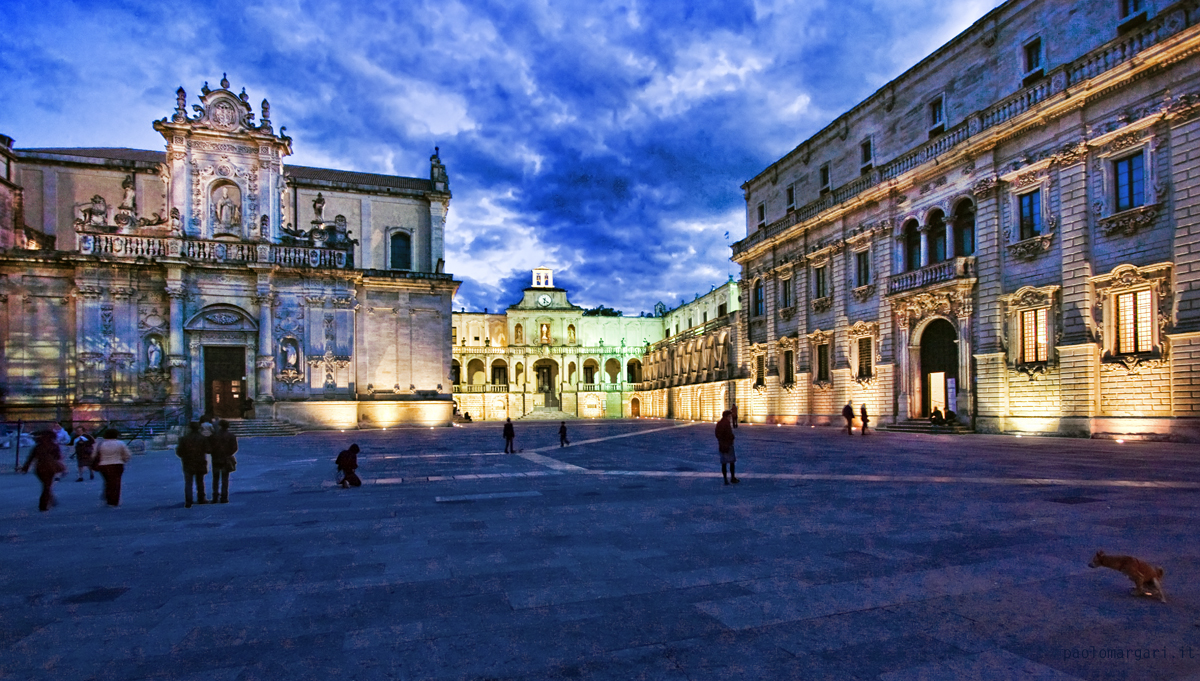
\includegraphics[height=1.05\paperheight]{Lecce1.jpg}};}
\begin{frame}
\centering
\footnotesize
\maketitle
\vspace{-.25cm}
\tiny{\textbf{Acknowledgements:} SeaDataNet, EMODnet Chemistry, \\
EMODnet Biology, STARESO}
\vspace{.125cm}

\begin{figure}
\centering

\includegraphics[width=.1\paperwidth]{gherlogo_transparent.PNG}\hspace*{.5cm}
\includegraphics[width=.1\paperwidth]{logo_ulg}\hspace*{.5cm}
\includegraphics[width=.1\paperwidth]{Logo_SeaDataNet_fond_transparent}\hspace*{.5cm}
\includegraphics[width=.07\paperwidth]{logo_emodnet}\hspace*{.5cm}
\includegraphics[width=.09\paperwidth]{Logo_Stareso}
\end{figure}

\end{frame}
}}
%-------------------------------------------------------------------------
